%Este trabalho está licenciado sob a Licença Creative Commons Atribuição-CompartilhaIgual 3.0 Não Adaptada. Para ver uma cópia desta licença, visite http://creativecommons.org/licenses/by-sa/3.0/ ou envie uma carta para Creative Commons, PO Box 1866, Mountain View, CA 94042, USA.

\documentclass[../livro.tex]{subfiles}  %%DM%%Escolher document class and options article, etc

%define o diretório principal
\providecommand{\dir}{..}

%%%%%%%%%%%%%%%%%%%%%%%%%%%%%%%%%%%%%%%%%%%%%
%%%%%%%%%%%%INICIO DO DOCUMENTO%%%%%%%%%%%%%%
%%%%%%%%%%%%%%%%%%%%%%%%%%%%%%%%%%%%%%%%%%%%%

\begin{document}

\chapter{Semana 2}

\vspace{0.5cm}

Existem maneiras diferentes de representar e de interpretar elementos de Álgebra Linear. Nesta parte, vemos algumas das principais.


\section{Vetores}

Um \textbf{vetor} no espaço tridimensional é um objeto com magnitude, direção e sentido bem definidos. Assim sendo, ao representar um vetor como na figura abaixo, não importa onde está o seu ponto inicial. Todas as setas representam o mesmo vetor.

\begin{figure}[h!]
\begin{center}
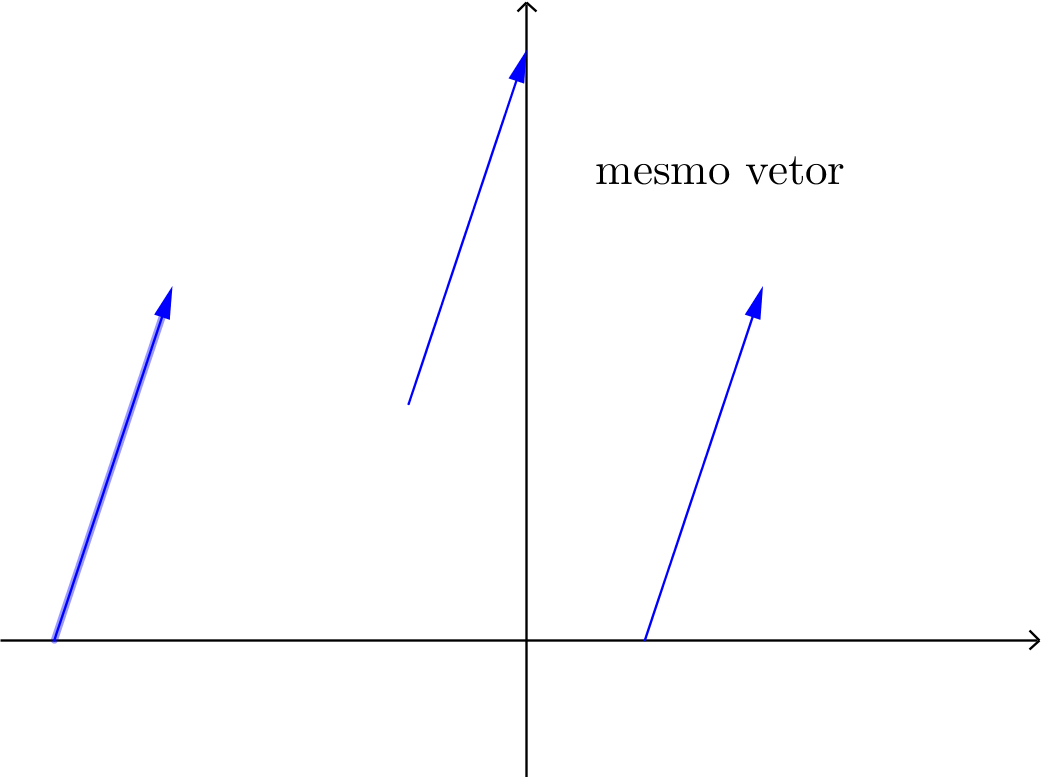
\includegraphics[width=0.3\linewidth]{\dir/Semana02/semana02-vetor}
\end{center}
\end{figure}

Fixando o sistema de coordenadas Cartesiano usual e usando a origem como referência, podemos introduzir coordenadas:
\[
\vec{v} =
\left[
  \begin{array}{c}
    v_1 \\
    v_2 \\
    v_3
  \end{array}
\right]
= v_1 \vec{e_1} + v_2 \vec{e_2} + v_3 \vec{e_3},
\] onde
\[
\vec{e_1} =
\left[
  \begin{array}{c}
    1 \\
    0 \\
    0
  \end{array}
\right], \quad
\vec{e_2} =
\left[
  \begin{array}{c}
    0 \\
    1 \\
    0
  \end{array}
\right] \quad  \text{e} \quad
\vec{e_3} =
\left[
  \begin{array}{c}
    0 \\
    0 \\
    1
  \end{array}
\right].
\] 


\noindent Intuitivamente, podemos pensar que o sistema de coordenadas Cartesiano fixa a origem como sendo o ponto inicial do vetor e o ponto $(v_1, v_2, v_3)$ do espaço tridimensional como o ponto final. 

\begin{figure}[h!]
\begin{center}
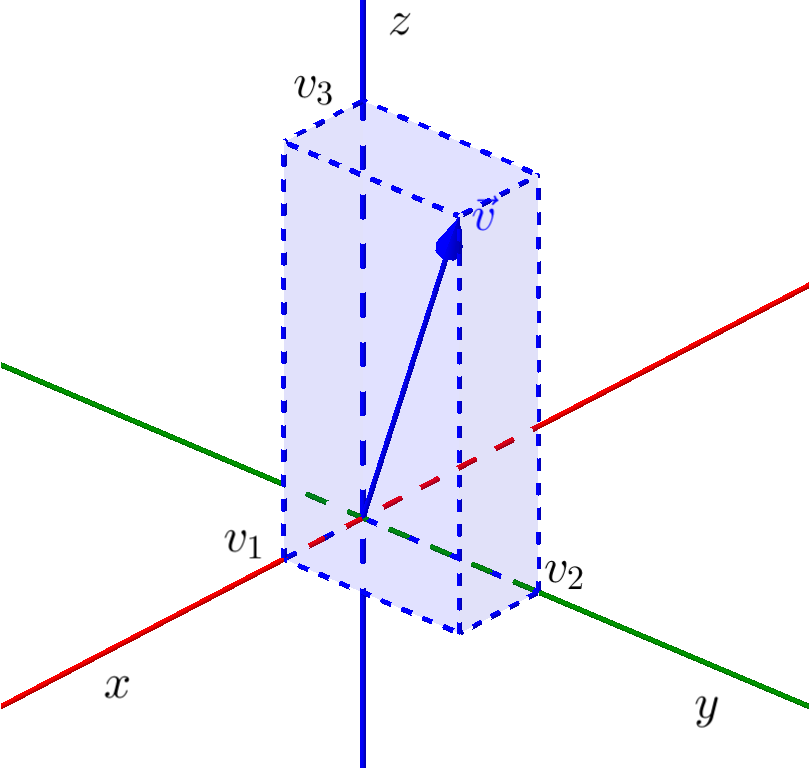
\includegraphics[width=0.2\linewidth]{\dir/Semana02/semana02-coord}
\end{center}
\end{figure}

No livro ``Álgebra Linear e suas Aplicações'', de David Lay, vetores são representados por letras em negrito. Nestas notas, utilizamos uma setinha em cima da letra para indicar um vetor.

Raramente vamos confundir o ponto $(v_1, v_2, v_3)$ com o vetor
\[
\left[
\begin{array}{c}
v_1 \\
v_2 \\
v_3
\end{array}
\right].
\] De qualquer maneira, é bom estar atento, pois outros textos podem fazê-lo.

O conjunto de todos os vetores com três componentes como acima é chamado de $\bR^3$ (leia-se ``erre três''). Em coordenadas, se tivermos
\[
\vec{v} =
\left[
  \begin{array}{c}
    v_1 \\
    v_2 \\
    v_3
  \end{array}
\right]  \quad  \text{e} \quad
\vec{w} =
\left[
  \begin{array}{c}
    w_1 \\
    w_2 \\
    w_3
  \end{array}
\right],
\] podemos definir a \textbf{soma de vetores} componente a componente:
\[
\vec{v} + \vec{w} :=
\left[
  \begin{array}{c}
    v_1 + w_1 \\
    v_2 + w_2 \\
    v_3 + w_3
  \end{array}
\right].
\] Geometricamente, isto pode ser interpretado como segue:
\begin{figure}[h!]
\begin{center}
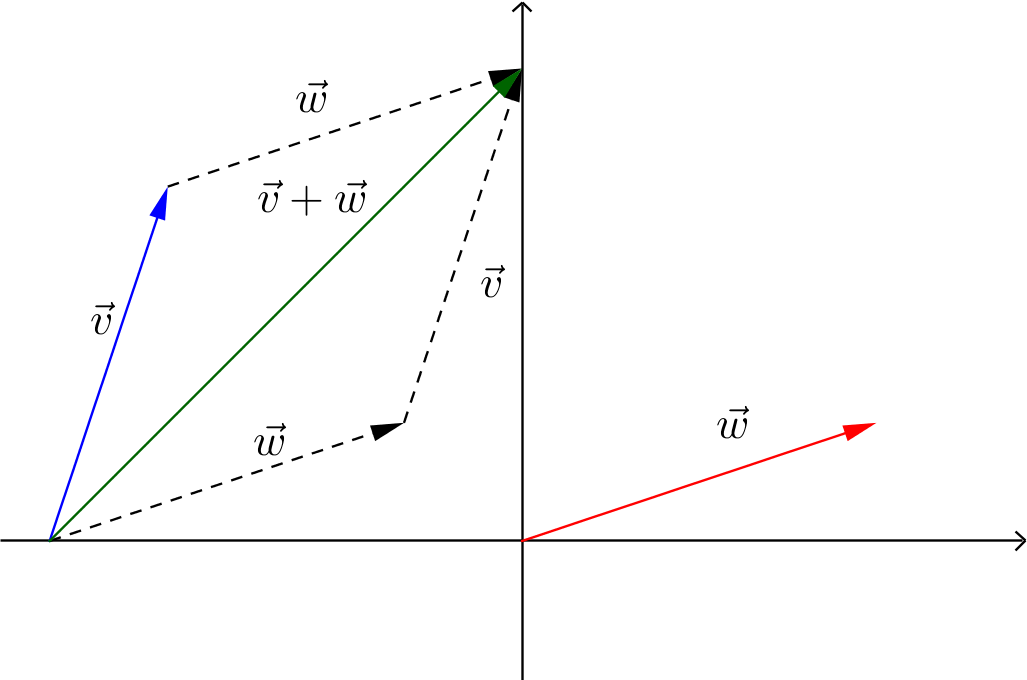
\includegraphics[width=0.3\linewidth]{\dir/Semana02/semana02-soma}
\end{center}
\end{figure}

A \textbf{multiplicação} do vetor $\vec{v}$ \textbf{por escalar} $k \in \bR$ é definida como:
\[
k \vec{v} :=
\left[
  \begin{array}{c}
    k v_1 \\
    k v_2 \\
    k v_3
  \end{array}
\right].
\] Geometricamente,
\begin{figure}[h!]
\begin{center}
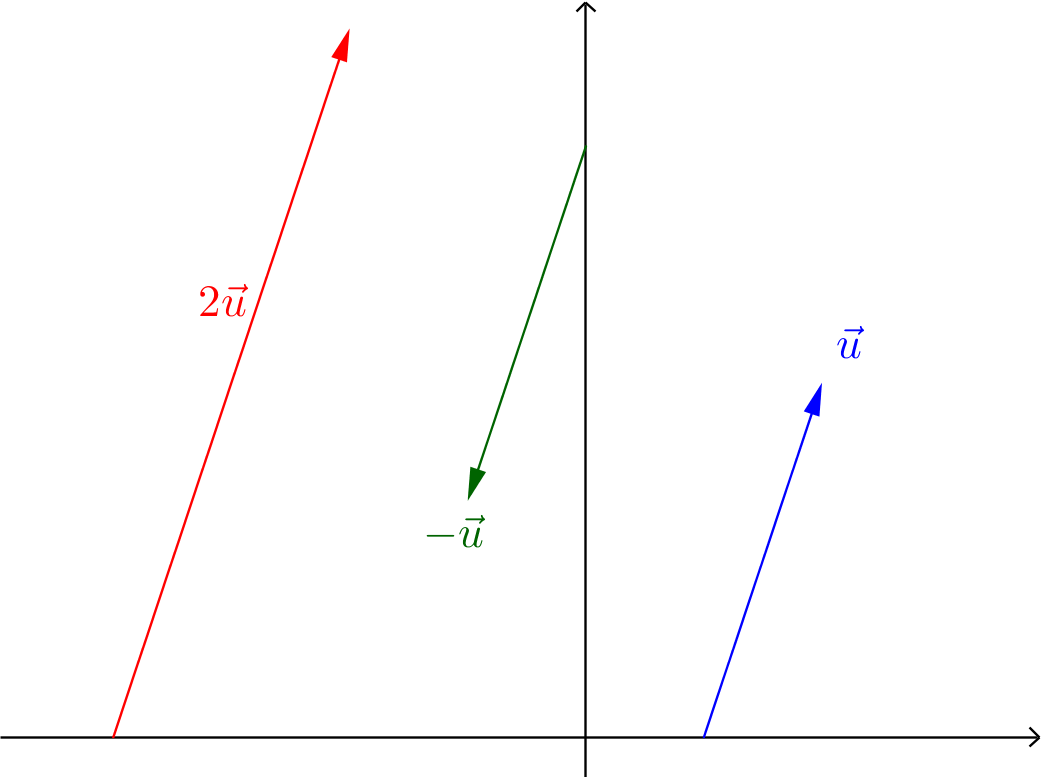
\includegraphics[width=0.3\linewidth]{\dir/Semana02/semana02-escalar}
\end{center}
\end{figure}



Estas considerações que fizemos também são válidas para outro número de componentes, com a possível perda de visualização geométrica, no caso de quatro ou mais componentes.

Mais geralmente, um vetor $\vec{v}$ do conjunto $\bR^n$ pode ser pensado como um objeto com $n$ componentes:
\[
\vec{v} =
\left[
  \begin{array}{c}
    v_1 \\
    v_2 \\
   \vdots \\
    v_{n-1} \\
    v_n
  \end{array}
\right]
= v_1 \vec{e}_1 + v_2 \vec{e}_2 + \cdots + v_{n-1} \vec{e}_{n-1} + v_{n} \vec{e}_{n},
\] onde
\[
\vec{e}_1 =
\left[
  \begin{array}{c}
    1 \\
    0 \\
  \vdots \\
    0 \\
    0
  \end{array}
\right], \quad
\vec{e}_2 =
\left[
  \begin{array}{c}
    0 \\
    1 \\
    0 \\
  \vdots \\
    0
  \end{array}
\right],   \cdots, \quad
\vec{e}_{n-1} =
\left[
  \begin{array}{c}
    0 \\
    0 \\
  \vdots \\
    1 \\
    0
  \end{array}
\right], \quad
\vec{e}_n =
\left[
  \begin{array}{c}
    0 \\
    0 \\
  \vdots \\
    0 \\
    1
  \end{array}
\right].
\] A soma de vetores é dada em coordenadas por:
\[
\vec{v} + \vec{w} :=
\left[
  \begin{array}{c}
    v_1 + w_1 \\
    v_2 + w_2 \\
    \vdots \\
    v_{n-1} + w_{n-1} \\
    v_n + w_n
  \end{array}
\right].
\] A multiplicação por escalar por:
\[
k \vec{v} :=
\left[
  \begin{array}{c}
    k v_1 \\
    k v_2 \\
    \vdots \\
    k v_{n-1} \\
    k v_n
  \end{array}
\right].
\]



\subsection{Representação matricial para sistemas Lineares}

Na linguagem da seção anterior, nós dizemos que dois vetores são iguais quando todas as suas componentes são iguais. Desta forma, podemos interpretar as equações de um sistema linear
\begin{equation*}
  \left\{
    \begin{array}{rcl}
      x+3y&=&1 \\
      2x-y&=&-2
    \end{array}
  \right.
\end{equation*} como uma igualdade entre vetores de $\bR^2$, isto é, de vetores com duas componentes:
\begin{equation*}
  \left[
    \begin{array}{c}
      x+3y \\
      2x-y
    \end{array}
  \right] =
    \left[
    \begin{array}{c}
      -1 \\
      2
    \end{array}
  \right].
\end{equation*} Além disso, é desta forma que surge naturalmente o \textbf{produto de uma matriz por um vetor}:
\begin{equation*}
  \left[
    \begin{array}{cc}
      1 & 3 \\
      2 & -1
    \end{array}
  \right]
  \left[
    \begin{array}{c}
      x \\
      y
    \end{array}
  \right] =
    \left[
    \begin{array}{c}
      -1 \\
      2
    \end{array}
  \right],
\end{equation*} definido de modo que as duas últimas igualdades acima signifiquem a mesma coisa. Esta última notação é conhecida como a \textbf{forma matricial} do sistema linear.




\begin{example}\label{example1}
O sistema, que já apareceu nas notas da semana anterior
\[
\left\{
  \begin{array}{ll}
    x_1 + 2x_2 + x_3 = 12 \\
    x_1 -3x_2 + 5x_3 = 1 \\
    2x_1 - x_2 + 3x_3 = 10
  \end{array}
\right.
\] pode ser representado matricialmente por
\[
\left[
  \begin{array}{ccc}
    1 &  2 & 1  \\
    1 & -3 & 5  \\
    2 & -1 & 3
  \end{array}
\right]
\left[
  \begin{array}{c}
    x_1   \\
    x_2  \\
    x_3
  \end{array}
\right] =
\left[
  \begin{array}{c}
    12   \\
    1  \\
    10
  \end{array}
\right].
\] De forma mais sucinta,
\[
\boxed{A \vec{x} = \vec{b}}
\] onde
\[
A = \left[
  \begin{array}{ccc}
    1 &  2 & 1  \\
    1 & -3 & 5  \\
    2 & -1 & 3  \\
  \end{array}
\right], \quad
\vec{x} = \left[
  \begin{array}{c}
    x_1   \\
    x_2  \\
    x_3
  \end{array}
\right], \ \text{ e } \
\vec{b} = \left[
  \begin{array}{c}
    12   \\
    1  \\
    10
  \end{array}
\right].
\] Chegamos a esta conclusão colocando os coeficientes da primeira variável $x_1$ na primeira coluna, os coeficientes da segunda variável $x_2$ na segunda coluna e os coeficientes da terceira variável $x_3$ na terceira coluna$. \ \lhd$
\end{example}


Mais geralmente, uma matriz do tipo $m\times n$ (leia-se ``$m$ por $n$'') é uma matriz com $m$ linhas e $n$ colunas:
\[
A = \left(a_{ij}\right) =
\begin{bmatrix}
a_{11}&a_{12}&\cdots &a_{1n}\\
a_{21}&a_{22}&\cdots &a_{2n}\\
\vdots &\vdots &\ddots &\vdots \\
a_{m1}&a_{m2}&\cdots &a_{mn}
\end{bmatrix}
\] e pode estar associada a um sistema com $m$ equações e $n$ variáveis, já que o produto
\[
\left[
  \begin{array}{cccc}
  a_{11}&a_{12}&\cdots &a_{1n}\\
  a_{21}&a_{22}&\cdots &a_{2n}\\
  \vdots &\vdots &\ddots &\vdots \\
  a_{m1}&a_{m2}&\cdots &a_{mn} \\
\end{array}
\right]
\left[
  \begin{array}{c}
    x_1 \\
    x_2 \\
    \vdots \\
    x_n
  \end{array}
\right] =
\left[
  \begin{array}{c}
    b_1 \\
    b_2 \\
    \vdots \\
    b_m
  \end{array}
\right],
\] quando visto componente a componente, representa:
\[
\left\{
  \begin{array}{cc}
  a_{11} x_1 + a_{12} x_2 + \cdots + a_{1n} x_n =  b_1 \\
  a_{21} x_1 + a_{22} x_2 + \cdots + a_{2n} x_n =  b_2 \\
    \vdots \\
  a_{m1} x_1 + a_{m2} x_2 + \cdots + a_{mn} x_n =  b_m \\
\end{array}
\right.
\]





\section{Combinações lineares de vetores}

Uma \textbf{combinação linear} dos vetores $\vec{v}_1, \vec{v}_2, \dots, \vec{v}_k$ é um vetor da forma:
\[
\vec{v} = x_1 \vec{v}_1 + x_2 \vec{v}_2 + \cdots + x_k \vec{v}_k = \sum_{i=1}^k x_i \vec{v}_i,
\] onde $x_1, x_2, \dots, x_k$ são números reais. Em outras palavras, uma combinação linear é uma soma de múltiplos dos vetores $\vec{v}_1, \vec{v}_2, \dots, \vec{v}_k$.


\begin{example}
Para os vetores
\[
\vec{v}_1 = \left[
  \begin{array}{c}
    1 \\
    -1
  \end{array}
\right] \quad \text{e} \quad
\vec{v}_2 = \left[
  \begin{array}{c}
    1 \\
    3
  \end{array}
\right],
\] algumas combinações lineares são:
\begin{itemize}
  \item $\vec{v}_1 + \vec{v}_2 =
  \left[
  \begin{array}{c}
    1 \\
    -1
  \end{array}
\right] +
\left[
  \begin{array}{c}
    1 \\
    3
  \end{array}
\right] =
\left[
  \begin{array}{c}
    2 \\
    2
  \end{array}
\right];$
  \item $ 4 \vec{v}_1 = 4 \vec{v}_1 + 0 \vec{v}_2 =
  4 \left[
  \begin{array}{c}
    1 \\
    -1
  \end{array}
\right] =
\left[
  \begin{array}{c}
    4 \\
    -4
  \end{array}
\right];$
  \item $ \vec{v}_2 = 0\vec{v}_1 + 1\vec{v}_2 =
   \left[
  \begin{array}{c}
    1 \\
    3
  \end{array}
\right];$
  \item $0\vec{v}_1 + 0 \vec{v}_2 =
  \left[
  \begin{array}{c}
    0 \\
    0
  \end{array}
\right] = \vec{0}.$
\end{itemize} \textbf{Geometricamente}, qualquer vetor do plano pode ser representado como combinação linear de vetores que não são colineares.

Vamos ilustrar este fato na figura abaixo.
\begin{figure}[h!]
\begin{center}
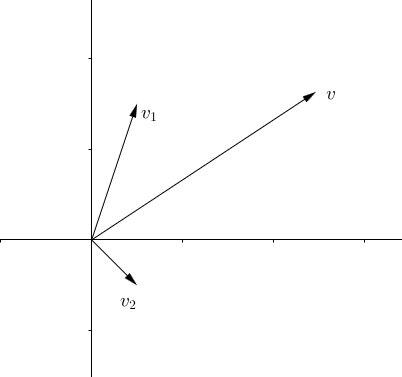
\includegraphics[width=0.4\linewidth]{\dir/Semana02/semana02-comblinear1}
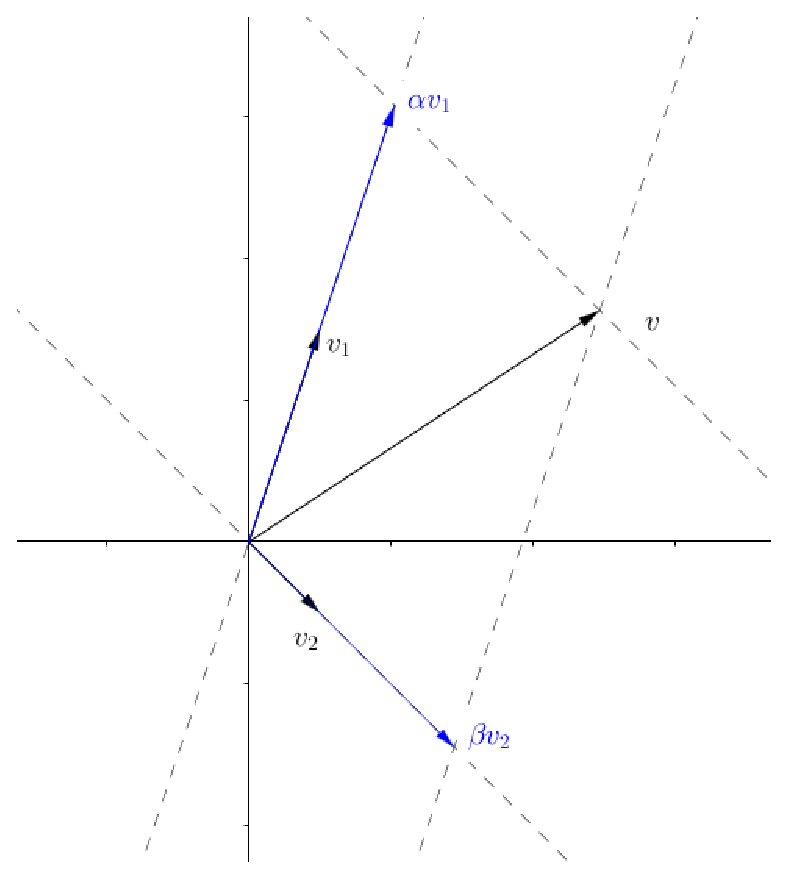
\includegraphics[width=0.4\linewidth]{\dir/Semana02/semana02-comblinear3}
\end{center}
\end{figure}
Por exemplo, para representar o vetor $\vec{v}$ como combinação linear de $\vec{v}_1$ e $\vec{v}_2$, podemos traçar retas paralelas aos vetores, passando pela origem e pela extremidade do vetor $\vec{v}$, como na figura da direita. Assim, pela interpretação geométrica da soma de vetores (ver início deste capítulo), sabemos que $\vec{v}$ é a soma dos vetores em azul. Mas estes, por construção, são colineares aos vetores iniciais e logo múltiplos destes. Concluimos que
\[
\vec{v} = \alpha \vec{v}_1 + \beta \vec{v}_2,
\] isto é, $\vec{v}$ é uma combinação linear de $\vec{v}_1$ e $\vec{v}_2$. $\ \lhd$
\end{example}



De forma mais geral, nós dizemos que um vetor $\vec{v} \in \bR^m$ é combinação linear dos $k$ vetores $\vec{v}_1, \vec{v}_2, \dots, \vec{v}_k  \in \bR^m$ quando conseguirmos encontrar números reais $x_1, x_2, \dots, x_k$ tais que
\[
x_1 \vec{v}_1 + x_2 \vec{v}_2 + \dots + x_k \vec{v}_k = \vec{v}.
\] Nós vamos nos referir a este tipo de equação por \textbf{equação vetorial}. Para decidir se um vetor é combinação linear de outros, devemos decidir se existem estes números reais $x_1, x_2, \dots, x_k$. Escrevendo em coordenadas:
\[
\vec{v}_1 =
\left[
  \begin{array}{c}
    v_{11} \\
    v_{21} \\
    v_{31} \\
    \vdots \\
    v_{m1}
  \end{array}
\right], \
\vec{v}_2 =
\left[
  \begin{array}{c}
    v_{12} \\
    v_{22} \\
    v_{32} \\
    \vdots \\
    v_{m2}
  \end{array}
\right], \
\vec{v}_3 =
\left[
  \begin{array}{c}
    v_{13} \\
    v_{23} \\
    v_{33} \\
    \vdots \\
    v_{m3}
  \end{array}
\right], \ \cdots, \
\vec{v}_k =
\left[
  \begin{array}{c}
    v_{1k} \\
    v_{2k} \\
    v_{3k} \\
    \vdots \\
    v_{mk}
  \end{array}
\right], \
\vec{v} =
\left[
  \begin{array}{c}
    b_{1} \\
    b_{2} \\
    b_{3} \\
    \vdots \\
    b_{m}
  \end{array}
\right],
\] vemos que encontrar os coeficientes da combinação linear, caso estes existam, equivale a resolver a equação vetorial
\[
x_1 \left[
  \begin{array}{c}
    v_{11} \\
    v_{21} \\
    v_{31} \\
    \vdots \\
    v_{m1}
  \end{array}
\right] + x_2
\left[
  \begin{array}{c}
    v_{12} \\
    v_{22} \\
    v_{32} \\
    \vdots \\
    v_{m2}
  \end{array}
\right] + x_3
\left[
  \begin{array}{c}
    v_{13} \\
    v_{23} \\
    v_{33} \\
    \vdots \\
    v_{m3}
  \end{array}
\right] + \cdots + x_k
\left[
  \begin{array}{c}
    v_{1k} \\
    v_{2k} \\
    v_{3k} \\
    \vdots \\
    v_{mk}
  \end{array}
\right] =
\left[
  \begin{array}{c}
    b_{1} \\
    b_{2} \\
    b_{3} \\
    \vdots \\
    b_{m}
  \end{array}
\right],
\] que, por sua vez, é equivalente a
\[
\left[
  \begin{array}{c}
   v_{11} x_1 + v_{12} x_2 + v_{13} x_3 + \cdots + v_{1k} x_k  \\
   v_{21} x_1 + v_{22} x_2 + v_{23} x_3 + \cdots + v_{2k} x_k  \\
   v_{31} x_1 + v_{32} x_2 + v_{33} x_3 + \cdots + v_{3k} x_k  \\
   \vdots  \\
   v_{m1} x_1 + v_{m2} x_2 + v_{m3} x_3 + \cdots + v_{mk} x_k
  \end{array}
\right] =
\left[
  \begin{array}{c}
    b_{1} \\
    b_{2} \\
    b_{3} \\
    \vdots \\
    b_{m}
  \end{array}
\right].
\] Mas isto é resolver um sistema linear! Portanto este conceito (aparentemente) novo está intimamente relacionado com tudo o que já tínhamos visto antes.


O \textbf{espaço gerado} por todas as combinações lineares dos vetores $\vec{v}_1, \vec{v}_2, \dots, \vec{v}_k$ é denotado por $\Span \{ \vec{v}_1, \vec{v}_2, \dots, \vec{v}_k \}$.

\begin{itemize}
\item Vimos que o conjunto gerado pelos dois vetores do exemplo anterior é o plano inteiro, isto é, $\Span \{ \vec{v}_1, \vec{v}_2 \} = \bR^2$.
\item Nota que o vetor nulo sempre pertence ao espaço gerado, assim como todos os vetores $\vec{v}_1, \vec{v}_2, \dots, \vec{v}_k$.
\item O conjunto gerado por apenas um vetor não nulo representa uma reta.
\end{itemize}



\section{Sistemas lineares e combinações lineares das colunas}

A associação feita acima pode ser resumida como:
% \[
% \boxed{\begin{eqnarray*}
% \text{Resolver o sistema linear $A \vec{x} = \vec{b}$ equivale a decidir se o} \\ \text{vetor $\vec{b}$ é uma combinação linear das colunas de $A$.}
% \end{eqnarray*}}
%\]
\begin{center}
  ''resolver o sistema linear $A \vec{x} = \vec{b}$ equivale a decidir
  se o vetor $\vec{b}$ é uma combinação linear das colunas de $A$''
\end{center}
ou ainda
\begin{center}
  ''resolver o sistema linear $A \vec{x} = \vec{b}$ equivale a decidir se o vetor $\vec{b}$ pertence ao espaço gerado pelas colunas de $A$''
\end{center}
% \[
% \boxed{\begin{split}
% \text{Resolver o sistema linear $A \vec{x} = \vec{b}$ equivale a decidir se o} \\ \text{vetor $\vec{b}$ pertence ao espaço gerado pelas colunas de $A$.}
% \end{split}}
% \]

Desta forma, tudo o que já vimos sobre existência de soluções para sistemas lineares pode ser ``traduzido'' para o contexto de combinações lineares e espaços gerados (faça as traduções!).


\begin{example}
Considere o sistema linear do Exemplo \ref{example1}:
\[
\left\{
\begin{array}{ll}
x_1 + 2x_2 + x_3 = 12 \\
x_1 -3x_2 + 5x_3 = 1 \\
2x_1 - x_2 + 3x_3 = 10
\end{array}
\right.
\] 
\begin{enumerate}[$(i)$]
\item Vimos ques este sistema pode ser representado em \textbf{forma matricial} por
\[
\left[
\begin{array}{ccc}
1 &  2 & 1  \\
1 & -3 & 5  \\
2 & -1 & 3
\end{array}
\right]
\left[
\begin{array}{c}
x_1   \\
x_2  \\
x_3
\end{array}
\right] =
\left[
\begin{array}{c}
12   \\
1  \\
10
\end{array}
\right].
\] Este formato é interessante principalmente para uma análise mais teórica. Podemos escalonar a matriz para decidir sobre a existência de soluções. Podemos também encarar o sistema como uma equação \textit{aparentemente} escalar $A \vec{x} = \vec{b}$; por exemplo, mais adiante no nosso curso, vamos tentar entender quando que pode fazer sentido escrever a solução como $\vec{x} = A^{-1} \vec{b}$; isto é o que se faria em uma equação linear escalar (adiantando: nem sempre se pode fazer isso!).
\item Também podemos representar o sistema como uma \textbf{matriz aumentada associada}:
\[
\left[
\begin{array}{ccc|c}
1 &  2 & 1 & 12 \\
1 & -3 & 5 &  1 \\
2 & -1 & 3 & 10
\end{array}
\right].
\] Esta notação é boa para a resolução do sistema. Escalonando a matriz aumentada associada, conseguiremos dizer se o sistema possui solução (no caso em que uma linha da forma escalonada for contraditória), se o sistema possui apenas uma solução (quando todas as colunas referentes às variáveis do sistema possuem posição de pivô) ou então se existem infinitas soluções (caso sem linhas contraditórias em que existem colunas sem posição de pivô -- assocaidas com variáveis livres).
\item Outra forma possível é a \textbf{forma vetorial} (equivalentemente \textbf{combinação linear das colunas} da matriz associada)
\[
x_1
\left[
\begin{array}{c}
1   \\
1  \\
2 
\end{array}
\right] + x_2 
\left[
\begin{array}{c}
  2   \\
 -3   \\
 -1
\end{array}
\right] + x_3 
\left[
\begin{array}{c}
 1  \\
 5  \\
 3
\end{array}
\right] = 
\left[
\begin{array}{c}
12   \\
1  \\
10
\end{array}
\right].
\] 

Esta maneira de representar o sistema é favorável para descrições geométricas, pois já vimos como interpretar geometricamente combinações lineares de vetores. Também será interessante futuramente no curso quando a imagem de transformações lineares.
\end{enumerate}  O entendimento dessas interpretações diferentes facilita (e muito!) o entendimento de vários conceitos que veremos mais adiante no nosso curso de Álgebra Linear.
% É importante que saibamos passar de uma representação para outra sem dificuldades.
\end{example}

\end{document} 
